\subsection{Валидация модели турбулентности с поправкой на кривизну линий тока}
\label{UDUCTComparison}

Эффективность поправки на кривизну линий тока к модели Ментера можно проверить, если сравнить результаты расчётов плоского течения в U-образном канале, выполненных при помощи модифицированной модели турбулентности, с экспериментальными данными Монсона и др., приведёнными в \cite{Monson}.

В \textit{таблице \ref{tableUDuct}} представлены геометрические параметры канала и граничные условия. Стенки полагаются адиабатическими, а на выходной границе задаётся постоянное относительное давление $P_{out} = 0$. При таких параметрах, число Рейнольдса для данного течения $Re = 10^5$.

\begin{figure}[h]
	\begin{minipage}{0.5\linewidth}
		\captionof{table}{Геометрия канала}
			\begin{tabular}{r l}
				\hline
				\label{tableUDuct}
				Высота & $H=3.81cm$ \\
				Длина канала & $L = 10H$ \\
				Внутренний радиус & $R_i = 1.91cm$ \\
				Внешний радиус & $R_o = 5.72cm$ \\
				Скорость на входе & $U_{in} = 32 m/s$ \\
				Температура на входе & $T_{in} = 264 K$ \\
			\end{tabular}
	\end{minipage}
	\hspace{2em}
	\begin{minipage}{0.4\linewidth}
		\begin{flushright}
		\includegraphics[scale=0.4]{UDuct}
		\caption{Геометрия канала}
		\end{flushright}
	\end{minipage}
\end{figure}

\begin{figure}[ht]
	\begin{minipage}{0.475\linewidth}
		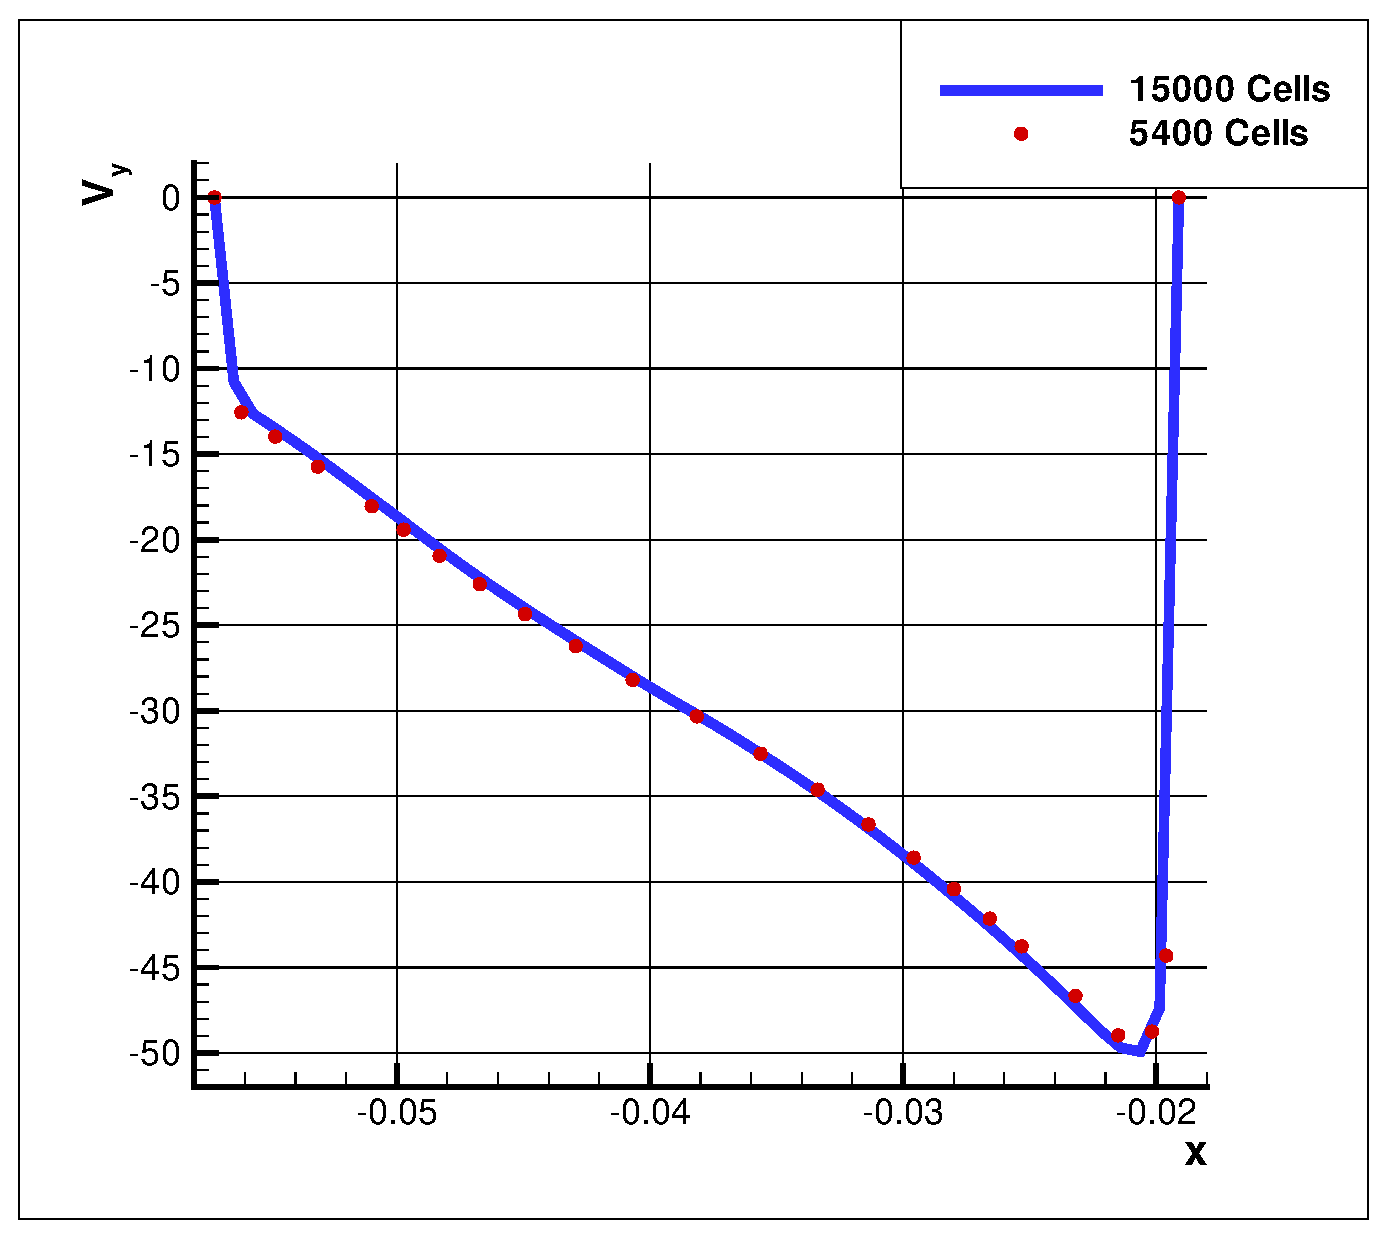
\includegraphics[scale=0.33]{uDuctMeshIndependence1}
		\caption{Сравнение графиков поперечной скорости на сетках 5400 ячеек и 15000 ячеек (FLUENT)}
		\label{fig:uDuctMeshIndependence1}
	\end{minipage}
	\hspace{0.5em}
	\begin{minipage}{0.475\linewidth}
		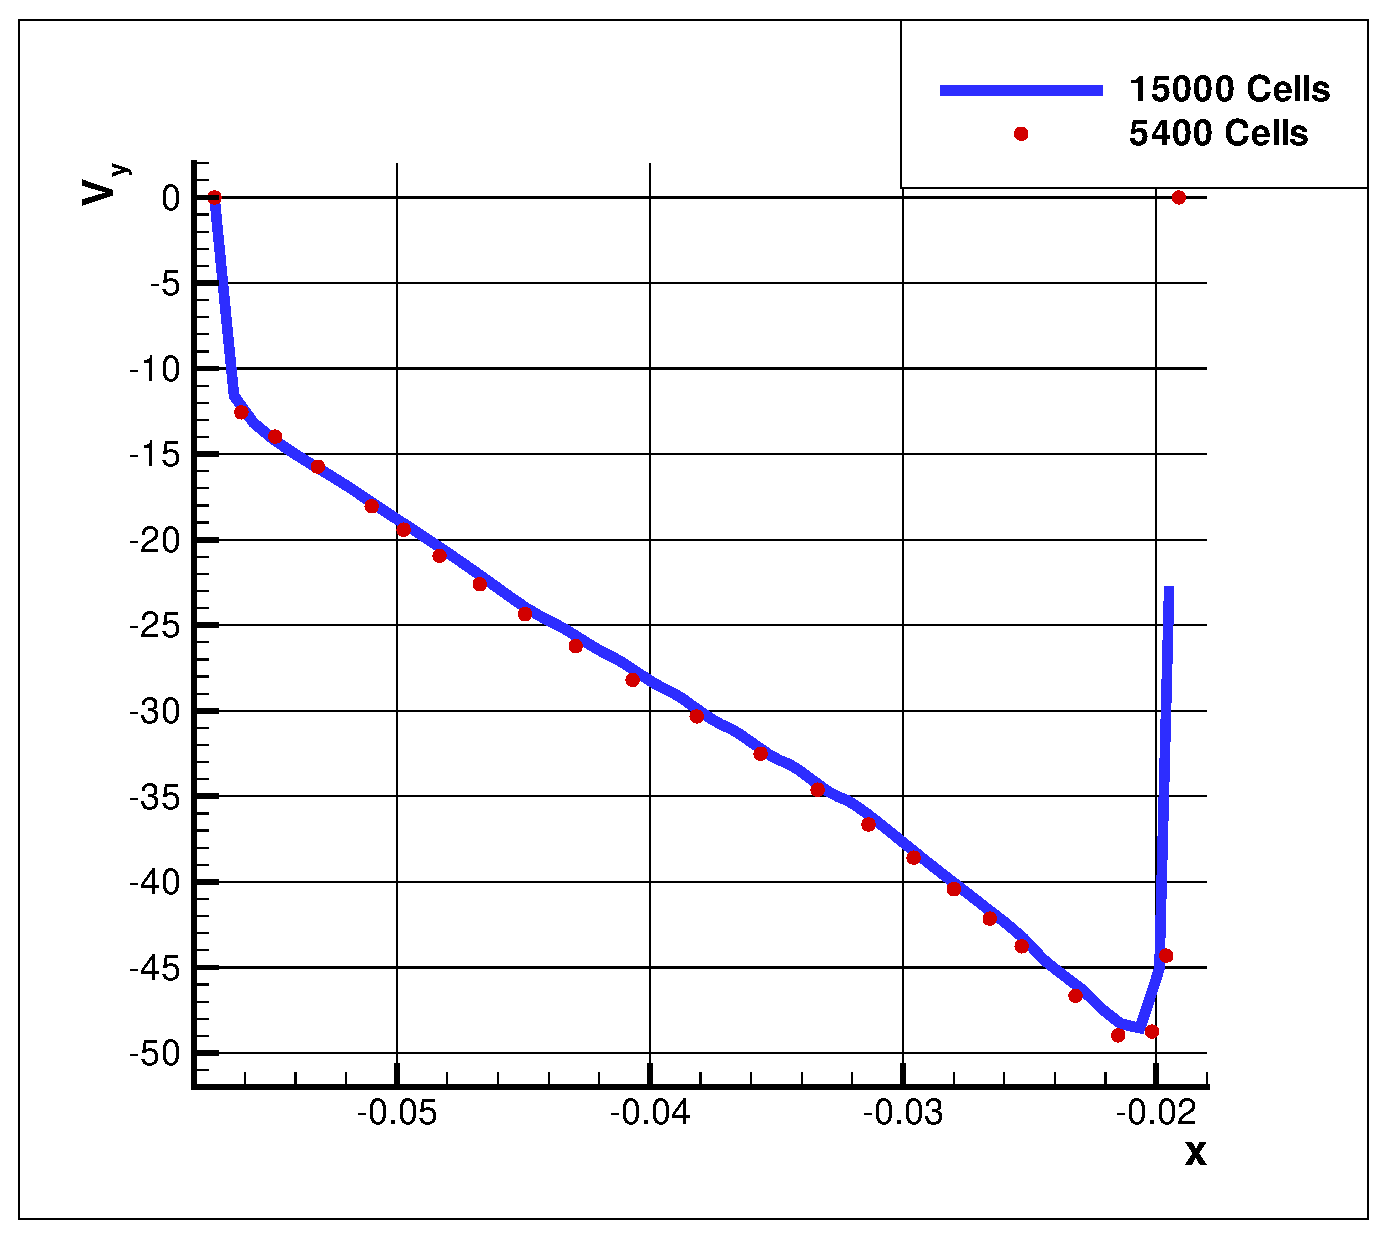
\includegraphics[scale=0.33]{uDuctMeshIndependence2}
		\caption{Сравнение графиков поперечной скорости на сетках 5400 ячеек и 15000 ячеек (OpenFOAM)}
		\label{fig:uDuctMeshIndependence2}
	\end{minipage}
\end{figure}
На \textit{рисунках \ref{fig:uDuctMeshIndependence1} и \ref{fig:uDuctMeshIndependence2}} показано сравнение решения на сетках 15000 ячеек и 5400 ячеек для поперечной компоненты скорости в сечении $y=0$. Очевидно, решения отличаютсяя менее, чем на $5\%$, что говорит о том, что сетки в 15000 ячеек достаточно для получения адекватного решения. Результаты далее приводятся для этой сетки.

\begin{figure}[h]
	\centering
	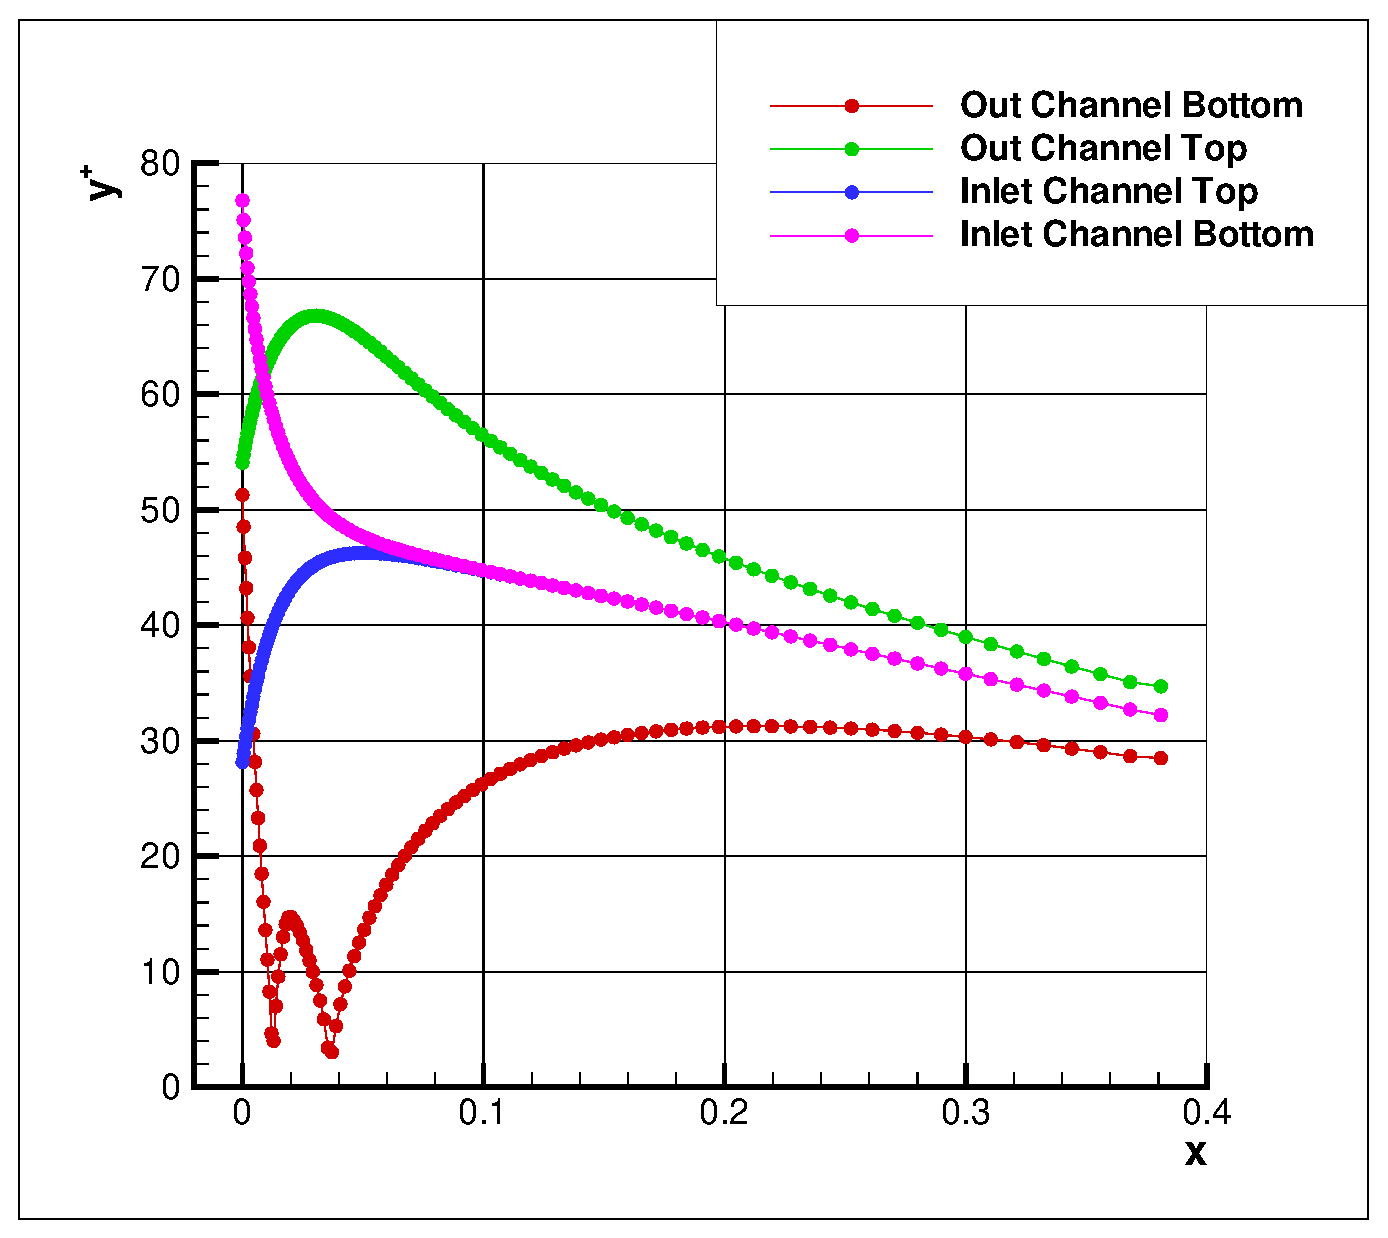
\includegraphics[scale=0.4]{uDuctyplus}
	\caption{Величина $y^{+}$ первой пристенной ячейки на внешней и внутренней стенках}
	\label{fig:uDuctyplus}
\end{figure}
	
Величина $y^{+}$ \textit{(рис. \ref{fig:uDuctyplus})} для первой пристенной ячейки (FLUENT) лежит в пределах $10 \div 80$, что вполне приемлемо для рассчётов с использованием автоматических пристеночных функций.